\subsubsection*{NRM}

\paragraph{Overview}

Argo Node Resource Manager (NRM) is a daemon running on the compute
nodes. It centralizes node management activities such as local application
launching, resource management, and power management.

NRM interacts with both global resource management services (e.g., job
scheduler) and with application components and runtime services running on
the node. It acts as a control infrastructure to enable custom resource
management policies at the node level.  Applications can influence these
mechanisms, both directly (through explicit API calls used, e.g., to
request additional resources on the node) and indirectly (by having their
run-time behavior monitored by NRM).

\paragraph{Key Challenges}

Many ECP applications have a complex runtime structure, ranging from in
situ data analysis, through an ensemble of largely independent individual
subjobs, to arbitrarily complex workflow structures.  At the same time, HPC
hardware complexity increases as well, from deeper memory hierarchies to
heterogeneous compute resources and performance fluctuating based on
power/thermal constraints.

Even in the common case of each compute node being allocated exclusively to
a single job, managing available node resources can be a challenge.  If a
compute node is shared among multiple job components (a likely scenario
considering the reduced cost of data transfers), these components---if
allowed to freely share node resources---could interfere with one another,
resulting in suboptimal performance.  It is the NRM's job to rein in this
complexity by acting as a coarse-grained resource arbitrator.

\paragraph{Solution Strategy}

NRM uses an active approach to resource management. Physical and logical
resources on the compute nodes are configured, discovered, and accounted for.
NRM can manage compute nodes and individual components of parallel workloads,
in the sense that it performs an active accounting of two types of interfaces
for those workloads: sensors and actuators. These abstracted components are
available through an upstream API which enables their discovery and management.

\begin{wrapfigure}[15]{r}{.58\textwidth}
%\vspace{-3.0em}
  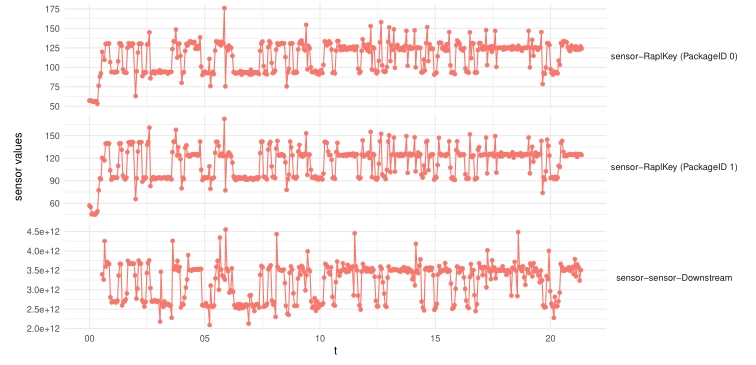
\includegraphics[width=.58\textwidth]{projects/2.3.1-PMR/2.3.1.19-Argo-PowerSteering/sensors}
  \caption{NRM sensor output.}
  \label{fig:argo-sensors}
\end{wrapfigure}

The NRM daemon supports power actuators, as well as sensors based on CPU counters
and power information. We also provide a simple API that application processes
can use to periodically update the NRM on their progress. This gives NRM
reliable feedback on the efficacy of its power policies, and it can also
be used for a more robust identification of the critical path, rather than
relying on heuristics based on performance counters.

In addition to those capabilities, NRM's configuration format allows for
the configuration of actuators and active polling sensors based on arbitrary
executables. Figure~\ref{fig:argo-sensors} shows a reading of NRM's sensor
outputs for two RAPL sensors along with CPU counter instrumentation. In order
to provide these capabilities, the NRM daemon manages the launching, management,
and stopping of parallel workloads through a unified interface. Resources
can be dynamically reconfigured at run time; these interfaces are provided
for use from applications and from global services.

\begin{wrapfigure}[12]{l}{.38\textwidth}
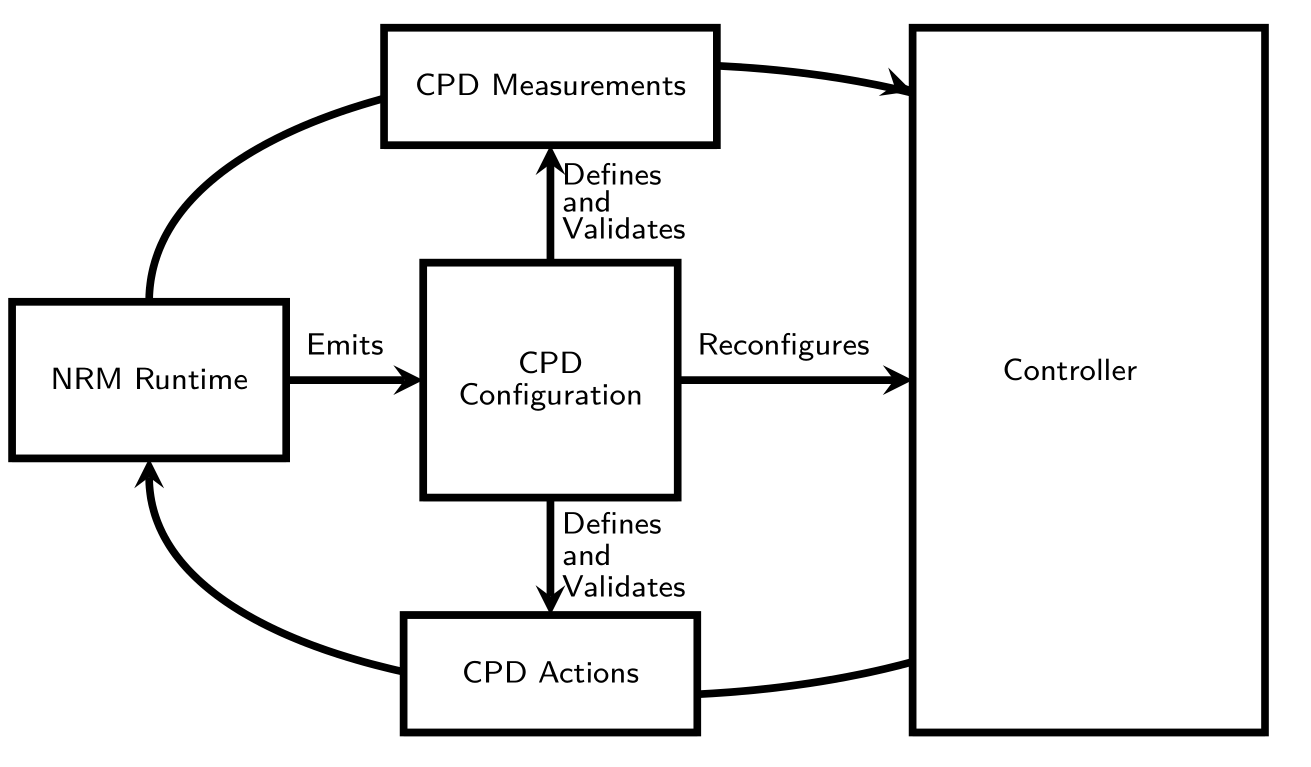
\includegraphics[width=.38\textwidth]{projects/2.3.1-PMR/2.3.1.19-Argo-PowerSteering/cpd}
\caption{Control Problem Description (CPD).}
\label{fig:argo-nrm-cpd}
\end{wrapfigure}
Other than sensor and actuator accounting capabilities, NRM provides
optional support for autonomic node management. This support is provided through
the accounting of node-local autonomic goals and constraints, which are
expressed in terms of available nodes and sensors. These goals and
constraints can be inspected by the users, global services (GRM), and
applications through NRM's unified interface. Inspection is achieved through
the emission of a Control Problem Description (CPD), which outlines active
sensors, actuators, goals, and constraints. This scheme is outlined in 
Figure~\ref{fig:argo-nrm-cpd}.

\paragraph{Recent Progress}

The NRM daemon continues to undergo major improvements in its interfaces to
interact with the rest of the system. This includes improvements to the
upstream API to allow for a passthrough mode, where NRM only manages the
collection of events from sensors and discovery and management of actuators
but does not enforce any control policy by itself. This passthrough mode
was used successfully to explore alternative control schemes inspired by
autonomic computing and a first integration with GEOPM (acting as the
global control loop across nodes). These efforts also led to the
improvement of the python interface offered by NRM.

We continue to improve our support for various sensors expected to be of
value on exascale systems, with the inclusion of an OMPT interface to
monitor OpenMP activity in controlled applications similar to our existing
PMPI support.

Our support for actuators is also growing, with the support for launching
an arbitrary command as an actuator, including the ability of the command
to receive information (pid) about an application as arguments.

We continue supporting the \texttt{libnrm} C library that can be linked to
applications in order to provide reports on application progress to NRM. We
have recently improved this interface to increase the resolution of the
timestamps associated with events, allowing for nanosecond precision in the
monitoring of fast events.

\paragraph{Preliminary Experiences on Early Access Systems}

We developed the Argo power management glue layer for Intel discrete GPUs
(APMIDG), which can communicate with NRM to manage the power consumption of
Intel discrete GPUs. It allows us to simultaneously measure the power
consumption, current frequency, and temperature of Intel discrete GPUs on
different domains (if available on target hardware). It also allows us to
control the power capping and the frequency range. We verified its power
management capabilities on Intel Arctic Sound GPUs, available as Aurora
Early Access Systems. In addition, we will verify the capabilities of Intel
Ponte Vecchio GPUs (Aurora GPUs) as soon as they become available. The
source code of APMIDG is maintained at \url{https://github.com/anlsys/apmidg},
which contains only public information.

\paragraph{Next Steps}

We are working on significantly improving the handling of sensor readings
(events) within the NRM. This includes gathering more metadata about the
physical location (on the topology) and scope (logic section of
code/thread/rank) that sensors report information about. We are also
looking into a more flexible mechanism to handle smoothing/integration of
sensor data across time: indeed, a critical component of any control loop
is its ability to understand how the system behaved since the last control
action. We are investigating possible designs to allow users to configure
how such integration should be done, as it currently only allows for
averaging data across time windows.

We are also working on slightly modifying the NRM infrastructure to allow
for it to be installed from Spack, delegating some of its privileged
operations to external tools (i.e., no admin rights needed anymore in the
core infrastructure).

We are planning to expand the list of resources managed by NRM by adding
support for other vendor-specific mechanisms as well.
